\newpage
\section{HTTP}
HTTP is a protocol that allows the user to request a \textbf{resource} (e.g. HTML page) that is on a server. They may contain references to other resources, therefore creating a \textit{web}, called \textbf{World Wide Web}.
\subsection{History}
The first idea came in 1945 by Vannever Bush, with his \textbf{Memtex}, a desk containing different information categorized accordingly: \textbf{hypertex} context was born. Then in 1962 Doug Engelbart started to work on its actual implementation and by 1989 Tim Berners Lee connected that with TCP/IP and DNS protocols, effectively creating the WWW. \\
Today it gives access to \textbf{intelinked documents} distributed across several computers in the world, using the internet as exchange.

\subsection{Communication}
\subsubsection{HTTP/1}
The standard way of communicating is between a \textbf{client} (e.g. Firefox, Chrome) and a \textbf{web server} (e.g. Apache, Nginx).\\
The communication is handled by the HTTP protocol (usually on port $80$). It's a text based \textbf{request/response} protocol.\\
It was \textbf{stateless} until version 2. This means that the server maintains no information about previous requests and thus the specification of the context is needed every time.\\

\paragraph{Request} HTTP requests follow the \textbf{REST} API principle, allowing for performance, scalability, simplicity, modifiability, portability and reliability. The resources are retrieved via a \textbf{URL}

\begin{center}
	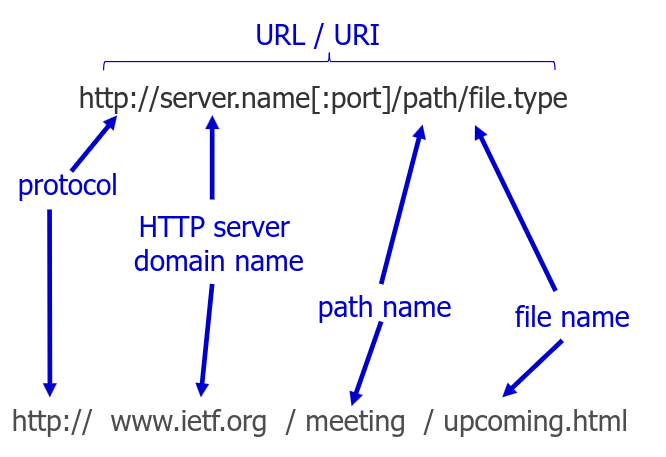
\includegraphics[scale=0.3]{url.png}
	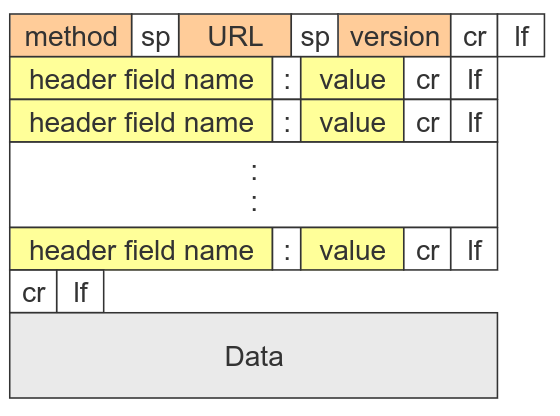
\includegraphics[scale=0.3]{httpreq.png}
\end{center}

\noindent The specified commands that can be used with a URL are:
\begin{itemize}
	\item \textbf{GET}: load a web page
	\item \textbf{HEAD}: load only the header of the web page, used for \textit{debugging}
	\item \textbf{PUT}: store a page on the web server
	\item \textbf{POST}: append something to the request passed to the web server
	\item \textbf{DELETE}: delete a web page
\end{itemize}

\newpage
\paragraph{Response}  The HTTP response contains the protocol used, the header lines and the \textbf{status code} , that can be:
\begin{itemize}
	\item \textbf{1xx}: only for information
	\item \textbf{2xx}: successful inquiry
	\item \textbf{3xx}: further activities are necessary
	\item \textbf{4xx}: client error (syntax)
	\item \textbf{5xx}: server error
\end{itemize}
\begin{center}
	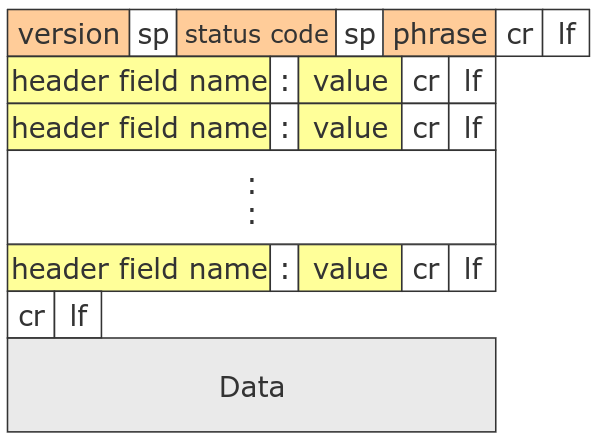
\includegraphics[scale=0.3]{httpresp.png}
\end{center}

\subsubsection{Web Sockets}
HTTP first problem is that the client needs to poll explicitly for content, causing a huge \textbf{overhead}. Thus Web Sockets were created: they allow a full duplex communication between the server and the client without the need of HTTP. It uses the same ports and it's set up using an HTTP request to "upgrade", which is then answered with a "switching protocol" response.

\subsubsection{WebRTC}
HTTP second problems is to enable communications between multiple browsers without creating a web server for each one of them. WebRTC implements a P2P communication that provides functions to establish media and data exchange, e.g. for videoconferencing.

\subsubsection{HTTP/2}
The second version of HTTP is \textbf{binary} instead of text based. It is fully \textbf{multiplexed}, associating requests and response and allowing a bi-directional stream. Therefore it can use only one connection while still granting \textbf{parallelism}. Furthermore it uses \textbf{header compression} to reduce overhead and allows server to push responses into client caches, reducing the number of requests to render web pages.
\begin{center}
	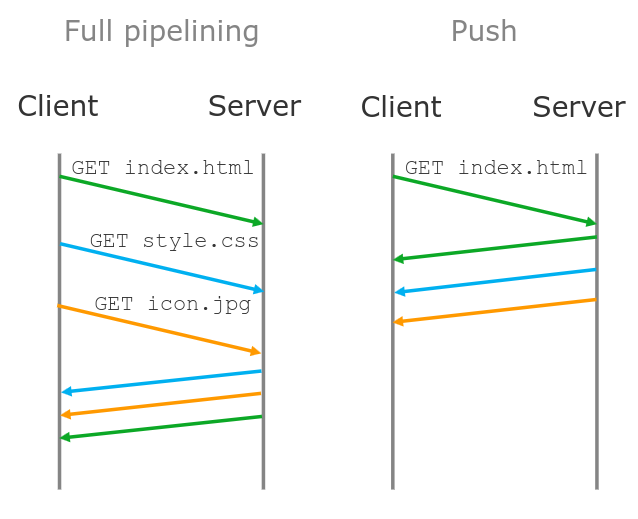
\includegraphics[scale=0.25]{http2.png}
\end{center}
\subsubsection{HTTP/3}
This version uses \textbf{QUIC} protocol over UDP instead of TCP and TLS for security, avoiding \textit{head of line} blocking.

\subsection{Cookies}
The main problem with HTTP is that it's \textbf{stateless}, this meaning that after every request/reply the web server forgets everything. While this is not a problem for simple browsing, it means that we cannot store user content to personalize the experience.\\
The solution is the \textbf{cookies}: tags stored in the web browser and set by the server so that they can be sent again to allow the latter to identify the client.\\
\subsubsection{Structure}
Cookies are stored as name-value pairs defined by the server. They can have optional parameters such as an \textbf{expiry date}.
\begin{center}
	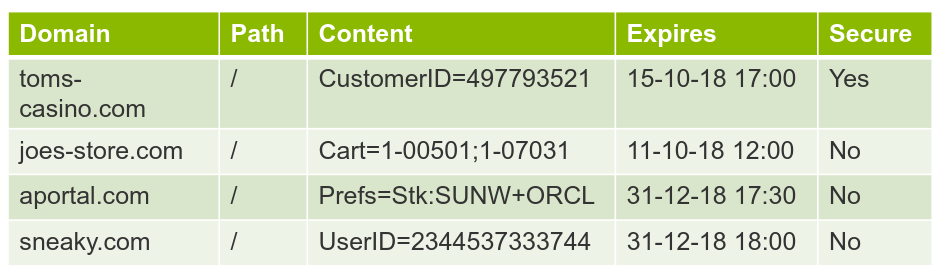
\includegraphics[scale=0.4]{cookies.png}
\end{center}

\subsubsection{Pros and cons}
They enable \textbf{authorization}, shopping carts, recommendations and \textbf{user session state} (e.g. for web mail). The biggest problem is about \textbf{privacy}: cookies are identified by \textbf{Etags}, an opaque identifier for a specific version of a resource, and can be used to track users.

\subsection{Proxy}
A \textbf{proxy} is an intermediate cache between multiple clients and a server. The main goal is to have a more \textbf{efficient} page loading, improving \textbf{scalability}. It temporarily stores the pages loaded by the browsers: if the client requests it and it hasn't changed yet, it's loaded from the proxy, otherwise a new request to the server is made and the cache is updated.\\
It can also enable support for protocols such as FTP or Telnet without the need for a new browser implementation.\\
It can also work as a \textbf{firewall}. 

\subsection{Scaling}
To handle huge loads (top 1000 websites) we use \textbf{3-tier} architecture, which separates the web server in \textbf{presentation servers}, \textbf{logic servers} and \textbf{database storage}. 
\begin{center}
	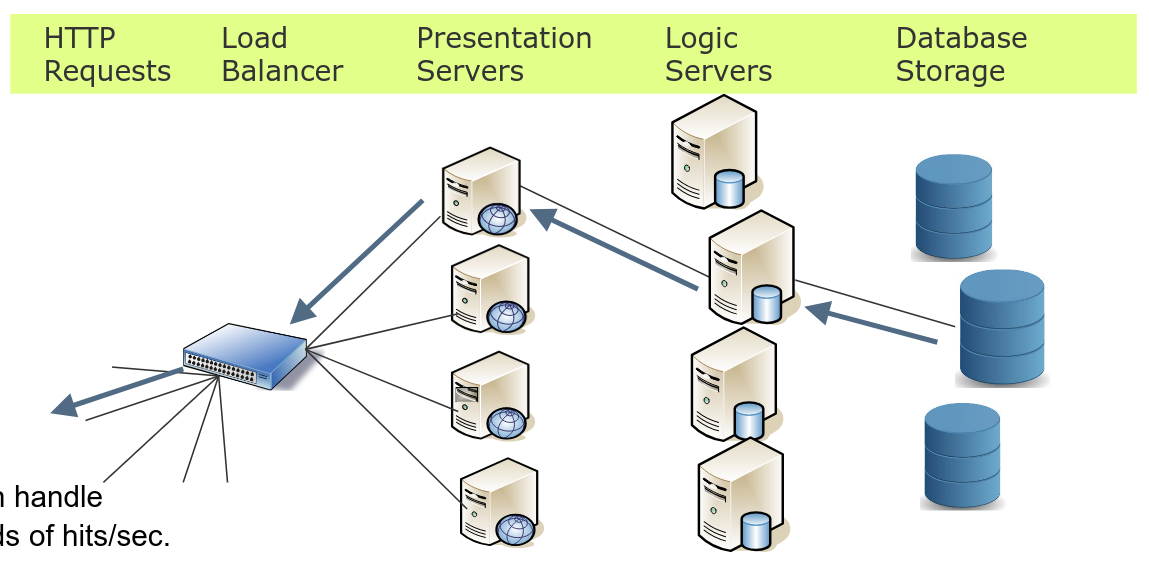
\includegraphics[scale=0.25]{3tier.png}
\end{center}
If, instead, we want to deal with medium and small web servers, we usually virtualize a lot of them on a single machine and we do the multiplexing with the server URL field in HTTP.

\subsection{DNS}
It's possible to use DNS over HTTP by sending a request (either \textit{GET} or \textit{POST}) to the DNS server. It improves privacy and security but the user looses control.